\chapter{Literature Review}
\label{ch:lit-review}
In this chapter an exploration of the current literature around direction finding is undertaken.
It will first cover an overview of the fundamentals of antenna arrays and signals in order to establish the concepts, terminology and mathematics required to understand specific DF techniques. 
Next, a variety of DF techniques will be analysed. The algorithm and principal of each technique will be presented, followed by the advantages and disadvantages of the technique. 
These advantages/disadvantages will be tied back to the user requirements defined in \Cref{ch:introduction} to ascertain whether the technique is appropriate for this application. Where possible, existing systems which implement a particular technique will be cited as examples.

The purpose of this chapter is to gain sufficient information about the various DF techniques to make informed system design decisions in \Cref{ch:system-design}, as well as to implement accurate simulations.

\subsection{Radio Frequency Signals and Antennas}
Some RF fundamentls used for modelling.

\section{Model from electronic warfare target location method}

The model which will be discussed here is that presented in \cite{poisel2012electronic}.  

Let there be an array of $M$ antenna elements receiving signals, where the position of of the \(m\)th element is \(\vec{x}_{m} = \begin{bmatrix}x_m & y_m & z_m \end{bmatrix}\).
The signal received by this \(m\)th element is influenced by the element position. 
This can be represented as \(\vec{r}_m(t, \vec{x}_m)\), showing that the signal at the \(m\)th element is a function of the position of the element.
As discussed by \cite{krim1996two}, this model contains both spacial and temporal information and hence is sufficient to be able to attain spacial information about the signal. 

It is further shown by Poisel that the delay time for a signal arriving at the \(m\)th sensor from a source located at azimuth angle \(\theta\) and elevation angle \(\phi\) is
\begin{align}
 \tau_m(\vec{\theta}) &= \tau_m ( \begin{bmatrix} \theta \\ \phi \end{bmatrix} ) \\
                       &= \frac{1}{c} [ x_m\cos(\theta)\cos(\phi) + y_m\sin(\theta)\cos(\phi) + z_m\sin(\phi) ]
\end{align}
This model assumes that the azimuth and elevation angle to the source, \(\begin{bmatrix}\theta & \phi\end{bmatrix}\TRANSPOSE\), is the same for each sensor. This is approximately true when the distance from the array to the source is much greater than the array geometry. Hence, it's often convenient and most accurate to select the center of the array as the origin. 
For a 2D space we let \(\phi = 0\) and hence simplify to:
\begin{equation}
 \tau_m(\theta) = \frac{1}{c} [ x_m\cos(\theta) + y_m\sin(\theta) ]
\end{equation}
Expressed as a matrix multiply:
\begin{align}
\tau_m(\theta) &= \frac{1}{c}\begin{bmatrix}x_m & y_m\end{bmatrix}\begin{bmatrix}\cos\theta\\ \sin\theta\end{bmatrix} \\
          &= \frac{1}{c} \vec{x}_m \vec{k}(\theta)
\end{align}
Where \(\vec{k}(\theta) = \begin{bmatrix}\cos\theta& \sin\theta\end{bmatrix}\TRANSPOSE\) is the wavenumber vector which graphically equates to the 'ratio' of how much the signal propagates in the x direction per distance propagated in the y direction. It's not really a ratio, it's a vector, so this doesn't quite makes sense. Note to self: tidy this up.

If this time delay is multiplied by the frequency in radians per second, \(\omega\), the result is the phase difference at the element relative to the origin:
\begin{align}
  \phi_m(\theta, \omega) &= \omega\tau_m(\theta) \\
                         &= \frac{\omega \vec{x}_m \vec{k}(\theta)}{c} \\
                         &= \frac{ \vec{x}_m \vec{k}(\theta) }{\lambda}
\end{align}

Representing the phase shift of all M sensors as a vector,
\begin{equation}
  \vec{\phi}(\theta, \omega) = \frac{\mathbf{X}\vec{k}(\theta)}{\lambda}
\end{equation}
Where \(\mathbf{X}\) is a \((M \times 2)\) matrix containing the \(x\) and \(y\) coordinates of each of the M sensors. 
In general, the output of an array is also impacted by the amplitude scaling and phase shifting applied to the received signals by the beam pattern of each sensor. The combination of the phase shift resulting from the physical separation of the sensors and the amplitude/phase response of a sensor is a very key property of an array known as the antenna array manifold, or steering vector, or source-position vector:
\begin{equation}
  \boxed{
    \vec{a}(\theta, \omega) = \vec{g}(\theta, \omega) \odot \exp \left\{ j \frac{\omega \mathbf{X} \vec{k}(\theta)}{c} \right\}
  }
\end{equation}

Often (as is the case in this project) the sensors used will be identical omnidirectional antennas. In this case, the amplitude and phase shift of the antennas as a result can be ignored, as it will be equal between elements and independent of angle or arrival. 
\begin{equation}
  \vec{a}(\theta, \omega) = \exp \left\{ j \frac{\omega \mathbf{X} \vec{k}(\theta)}{c} \right\}
\end{equation}

Or, more verbose:
\begin{align}
\vec{a}(\theta, \omega) &= \exp \left\{ \frac{j \omega}{c} \begin{bmatrix} x_1, y_1 \\ x_2, y_2 \\ .., .. \\ x_M, y_M \end{bmatrix} \begin{bmatrix} \cos(\theta) \\ \sin(\theta) \end{bmatrix} \right\} \\
                        &= \exp \left\{ \frac{j \omega}{c} \begin{bmatrix} x_1\cos(\theta) + y_1\sin(\theta) \\ x_2\cos(\theta) + y_2\sin(\theta)) \\ .., .. \\ x_M\cos(\theta) + y_M\sin(\theta) \end{bmatrix} \right\} \\
\end{align}

The vector output of the array, \(\vec{r}(t)\), where each element of the vector is the signal received by the sensor is the where each element of the vector corresponds to an antenna element is equal to the sum of the signals at that element by the principle of superposition. Algebraically:
\begin{equation}
  \vec{r}(t) = \sum_{k=1}^{K} s_k(t)\vec{a}_k(\vec{\theta}_k) + \vec{n}(t)
\end{equation}
Where:
\begin{itemize}
  \item \(s_k(t)\) is the source signal,
  \item \(\vec{\theta}_k = \begin{bmatrix} \phi_k, \theta_k \end{bmatrix}\TRANSPOSE\) is the source parameter vector, a vector with azimuth and elevation angles pointing in the direction of the source,
  \item \(\vec{a}_k(\vec{\theta}_k)\) is the antenna array manifold, explored more shortly,
  \item \(\vec{n}(t)\) is additive noise.
\end{itemize}

Or in matrix notation:
\begin{align}
  \vec{r}(t) = \mathbf{A}(\vec{\theta})\vec{s}(t) + \vec{n}(t)
\end{align}

The array manifold vector is also known as source position vector or as the steering vector. It is the response of the array to a signal impinging on the array from a certain azimuth and elevation angle, \((\phi, \theta)\). The response is naturally in terms of the gain and phase shifts introduced by each sensor as a result of the beam pattern and physical separation of the sensors. It is given by:
\cite{dacos1995estimating}.
\begin{equation}
\vec{a}(\theta, \phi) = \vec{g}(\theta, \phi) \odot \exp \left\{ -j \mathbf{X}\TRANSPOSE \vec{k}(\theta,\phi) \right\}
\end{equation}
Where:
\begin{itemize}
  \item \(\vec{g}(\theta, \phi)\) is a \(N\)-dimensional vector of complex number being the gain and phase response  of each element in the direction \((\theta, \phi)\). 
\item \(\mathbf{X}\TRANSPOSE\) is a \((N \times 3)\) matrix containing the \(x\), \(y\) and \(z\) coordinates of each of the N elements of the form \(\begin{bmatrix} \vec{x}, \vec{y}, \vec{z} \end{bmatrix}\TRANSPOSE\)
\item \(\vec{k}(\theta, \phi)\) is the wavenumber vector given by \(\vec{k}(\theta, \phi) = \pi \begin{bmatrix} \cos\theta\cos\phi, \sin\theta\cos\phi, \sin\phi \end{bmatrix}\TRANSPOSE \). Graphically, this equates to the 
\end{itemize}
For the purposes of this research the elements will all be located at the same elevation as we only with to locate terrestrial signals. Hence, this may be simplified to:
\begin{equation}
  \vec{a}(\theta) = \vec{g}(\theta) \odot \exp \left\{ -j \mathbf{X}\TRANSPOSE \vec{k}(\theta) \right\}
\end{equation}
Here, \(\mathbf{X}\TRANSPOSE\) is now a \((N \times 2)\) matrix of the form \(\begin{bmatrix} \vec{x}, \vec{y} \end{bmatrix}\) and \(\vec{k}(\theta) = \pi[\cos(\theta), \sin(\theta)]\TRANSPOSE\).

Furthermore, the \(\vec{g}\) term may be excluded if we assume omnidirectional elements. Although it is rare to deal with true omnidirectional antennas, for an antenna which is required to receive signals only in the azimuth plane, omnidirectional antennas such as dipoles might very well be used in practice. This hence simplifies to:

\begin{equation}
  \vec{a}(\theta) = \exp \left\{ -j \mathbf{X}\TRANSPOSE \vec{k}(\theta) \right\}
\end{equation}



The antenna array manifold can now be re-written:
\begin{align}
\vec{a}(\theta) &= 
  \exp \left\{ -j \begin{bmatrix} 
      \omega_c \tau_1(\phi_k)\\ 
      \omega_c \tau_2(\phi_k)\\ 
      \omega_c \tau_M(\phi_k) 
   \end{bmatrix} \right\} \\
  &= \begin{bmatrix}
      e^{-j\omega_c \tau_1(\phi_k)} \\
      e^{-j\omega_c \tau_2(\phi_k)} \\
      ... \\
      e^{-j\omega_c \tau_M(\phi_k)} \\
   \end{bmatrix}
\end{align}

Clearly, this is simply a vector of phase shifts introduced by each element in the array as a function of both the location of the element and the angle of the incident wave relative to some defined zero location and zero direction. It is said by \cite{dacos1995estimating} that this array manifold completely characterises the array. That paper goes into additional details on how the manifold may simplified for linear arrays, as well as the special properties which a manifold of a linear array possesses. This will not be discussed here as the array used for this DF system is not likely to be linear. 

Let there be $K$ individual signal sources, where $\vec{s}(t)$ represents the resultant signal, being
\begin{equation}
\vec{s}(t) = \begin{bmatrix} s_{1}(t) & s_{2}(t) & s_3(t) & ... & s_K(t) \end{bmatrix}
\end{equation}

This important result shows us that for a known array with omnidirectional antennas at arbitrary \(x)\) and \(y\) locations, receiving a narrow band signal of known frequency from a certain direction, \(\theta\), the phase shift at each element is a vector which can be easily calculated. This is the basis around which the direction finding algorithm for this project will be designed. 

\section{Direction Finding Techniques}
A direction finder is a passive device able to ascertain the angle of arrival of a source of electromagnetic radiation.
The objective of direction finding is generally to find the location of non-cooperative emitters\cite{poisel2012electronic}.
This is one of the fundamental activities of electronic defense as well as RFI hunting.
The general structure of a direction finding system is an antenna array connected to a receiver connected to a processing module connected to a display providing output to operators.
Simple direction finding systems were used as early as the start of the \nth{20} century and have been continually evolving since then along with developments in communications and electronic warfare systems.
Direction finding systems have applications in a variety of applications, ranging from radar, sonar, surveillance, radio astronomy and even medical. Finding an optimal parameter estimator for angle of arrival is difficult and hence lots of research has been done into the topic over the last few decades\cite{van2004detection}.

DF techniques are generally based on either amplitude comparison, time/phase comparison or statistical methods\cite{tuncer2009classical}. 
Various implementations of these classes of DF will now be explored.

Much of following overview of types of direction finding systems is based on discussions in the Electronic Warfare and Radar Systems Engineering Handbook\cite{center2012electronic}.

\subsection{Scanned beam}
This is a direct amplitude technique. An antenna with gain (non-uniform beam) is rotated and this causes the power output of the antenna to vary with rotation angle. This is the earliest form of direction radio direction finding and was implemented in the early 1900's. 
One of the first uses of this DF technique was in a system developed by Marconi to locate the bearing to a ship which was transmitting a signal for navigation purposes\cite{jenkins1991smallaperture}. A loop antenna was frequently used as it was a simple antenna to construct and the beam pattern has a sharp null. 
An example antenna and beam pattern are shown in \Cref{fig:lit_loop_antenna}. As the change in antenna output power per degree rotated is highest around the null, the antenna was often aligned such that the signal of interest was in the null. 
If multiple signals originating from different bearings are present, the system cannot operate. 
While today it may be possible to put highly selective receivers on the output of the antenna, this technology did not exist when scanning beam DF systems were originally used.

Note that as the beam pattern is symmetric about both the \(x\) and \(y\) axis, there are in general 4 ambiguous points. However, if the antenna can be rotated such that the signal is in the null, there is then only 2 ambiguous points, or \SI{180}{\degree} ambiguity. This ambiguity can be resolved with an  additional antenna element. Note also that this is not an instantaneous DF technique as it requires time for the antenna to be rotated. Hence, this technique is not suitable for finding transients. 

Loop antennas DF systems are very sensitive to multipath errors, especially ionospheric reflection \cite{jenkins1991smallaperture}. 
\begin{figure}
  \centering
  \begin{subfigure}[b]{0.48\textwidth}
    \centering
    \includegraphics[width=0.8\textwidth]{lit_review/loop_antenna}
    \caption{Loop antenna used for direction finding in 1918. Src: \cite{grabau1989funkpeiltechnik}}
  \end{subfigure}
  ~
  \begin{subfigure}[b]{0.48\textwidth}
    \centering
   \includegraphics[width=0.7\textwidth]{lit_review/loop_antenna_beam}
   \caption{Beam pattern of loop antenna or dipole. Note the sharp null. Src: \cite{jenkins1991smallaperture}}
  \end{subfigure}
  \caption{Loop antenna and beam pattern}
  \label{fig:lit_loop_antenna}
\end{figure}

\subsection{Crossed Loop}
The crossed loop technique is an amplitude comparison technique. 
As is shown in \Cref{fig:lit_crossed_loop_antenna}, using two loop antennas perpendicular to one another produces two beam patterns: one being proportional to the sine of the angle and the other to the cos of the angle. 
By comparing the signal power from each antenna, it is possible to ascertain the \gls{aoa}. This system is instantaneous as only a single pulse is necessary to ascertain the ratio of antenna output power. However it has many ambiguities. Some ambiguities can be resolved with a sense antenna. 
For optimal ambiguity resolution, the crossed loop should be rotated such that signal of interest is located in the null of one of the loops and the peak of the other. This resolves ambiguity but at the expense of the system not being real-time.
As with the scanned beam, the crossed loop suffers from significant performance degradation arising from multipath, specifically ionospheric reflection. 
In the 1930's a marine radio direction finder network using the crossed loop amplitude comparison technique was set up for marine navigation. Then, during World War II, rapid improvements to DF technology were made with the operating frequency of the systems being extended into the VHF and UHF band  and extensive DF networks being installed\cite{jenkins1991smallaperture}. The tactical advantage which DF systems provided prompted significant development into DF during the war.
\begin{figure}
  \centering
  \begin{subfigure}[b]{0.3\textwidth}
    \includegraphics[width=\textwidth]{./img/lit_review/loop_antenna_crossed}
    \caption{Example of crossed loop antenna.}
  \end{subfigure}
  ~
  \begin{subfigure}[b]{0.4\textwidth}
    \includegraphics[width=\textwidth]{./img/lit_review/loop_antenna_crossed_beam}
    \caption{Crossed loop antenna beam pattern showing difference in magnitude seen by each loop. Src: \cite{jenkins1991smallaperture}}
  \end{subfigure}
  \caption{Crossed loop antenna and beam pattern}
  \label{fig:lit_crossed_loop_antenna}
\end{figure}

\subsection{Adcock Array}
The Adcock array was developed and patented in 1919 by British army engineer Frank Adcock \cite{gething1991radio}.
Instead of using loop antennas, the Adcock array makes use of two orthogonally orientated (crossed) pairs of monopole or dipole antennas. Typically a North-South pair and an East-West pair are used. These antenna pairs produce the same beam pattern as the loop antennas. 
As a loop antenna can be modeled by two vertical antennas on the sides and two horizontal antennas on the top and bottom of the loop, it should be clear that the loop is not polarisation selective. While the direct beam from the signal source may be vertically polarised, the reflected beam from atmospheric reflection was also being received and corrupting the signal output of the array.
The Adcock array which uses only vertical elements maintains the same beam pattern as the loop but is not sensitive to horizontally polarised radiation hence offers better performance for a DF system.
The antenna configuration of Adcock and Watson-Watt is shown in \Cref{fig:lit_adcock_array}.
This array configuration was studied extensively in the 1930's and played a significant role in the electronic warefare of World War II \cite{gething1991radio}. One of the advantages of it at the time was that the output it provided allowed it to directly drive a CRT display, giving the user real-time visibility into what the system was receiving\cite{jenkins1991smallaperture}. 

\begin{figure}
  \centering
  \begin{subfigure}[b]{0.25\textwidth}
    \includegraphics[width=\textwidth]{./img/lit_review/adcock_model}
  \end{subfigure}
  ~
  \begin{subfigure}[b]{0.6\textwidth}
    \includegraphics[width=\textwidth]{./img/lit_review/adcock_implementation}
  \end{subfigure}
  \caption{Left: model for adcock antenna showing N-S and E-W pairs. Right: Japanese implementation of array for 2 MHz direction finding. Src: \cite{japanesecommunications}}
  \label{fig:lit_adcock_array}
\end{figure}


\subsection{Watson-Watt Evaluation}
This amplitude comparison technique is probably the most commonly used DF technique over the history of DF systems\cite{poisel2012electronic}.

Ambiguity and multipath are one of the major difficulties which need to be overcome in direction finding systems. 
In the mid 1920s, Sir Robert Watson-Wat developed an improved DF system based on the Adcock array configuration. 
As discussed above, the beam pattern of the output of an Adcock array is one cosine shaped beam and one sine shaped beam. By exploiting the trigonometric properties of these functions and adding an additional sense element, Watson-Watt developed a method to compute the angle of arrival from an array with this cos/sin property. 
This evaluation technique showed significant improvement in rejection of ionospheric reflections and made ambiguity resolution easier.
In the case of Wattson-Watt, the beams are synthesised by forming sum and difference channels from broad beam antennas in an array.

The mathematics around this technique will not be explored in detail here, but a graphical view of the antenna and receiver structure can be seen in \Cref{fig:watson-watt}.
For a more detailed discussion of the mathematics behind the Watson-Watt DF algorithm, see Poisel\cite{poisel2008introduction}.
For a simulation of Watson-Watt algorithm as well as a discussion around an ambiguity resolution implementation using a sense antenna see Pellejero\cite{adcockwatsonwattrdf}.

\begin{figure}
  \centering
  \begin{subfigure}[b]{0.48\textwidth}
    \includegraphics[width=\textwidth]{./img/lit_review/watson-watt-processing-analogue}
    \caption{View showing transformer configuration to produced required difference signals. Src: \cite{poisel2008introduction}}
  \end{subfigure}
  ~
  \begin{subfigure}[b]{0.48\textwidth}
    \includegraphics[width=\textwidth]{./img/lit_review/watson-watt-processing-digital}
    \caption{Abstraced view of signal chain for digital processing. Src: \cite{rhode2000introtodf}}
  \end{subfigure}
  \caption{Watson-Watt array processing technique using the Adcock array. Note that difference channels from crossed beams are formed}
  \label{fig:watson-watt}
\end{figure}

\subsection{Doppler}
By the principle of Doppler shift, moving an antenna towards a signal source increases the observed frequency while moving an antenna away from a source lowers the observed frequency. 
If an antenna is rotated around a central point (tracing out the circumference of a circle), there will be 
The Doppler shift is given by: \cite{poisel2012electronic}
\begin{equation}
  \Delta f = \frac{B\omega}{c}f_c\sin(\Uppsi)
\end{equation}
Where \(B\) is the length of the antenna baseline, \(\omega\) is the angular velocity of the antenna, \(f_c\) is the carrier frequency of the signal source and \(\Uppsi\) is instantaneous difference between the angle towards the signal source and the angle of the rotating antenna (this is shown graphically in \Cref{fig:lit-review-doppler-switching}). By rotating one antenna around a reference antenna and measuring the received signal frequency difference, the Doppler shift can be measured and with the above equation the AoA calculated.

However, to DF a \SI{100}{\mega\hertz} tone with a Doppler shift of \SI{3}{\mega\hertz}, the antenna would need to be rotated with a tangential velocity of 10000 m/s\cite{jenkins1991smallaperture}. 
It is not practical to rotate an antenna at such a high speed. 
Hence, rather than physically rotating an antenna, what is done in practice is that a Doppler shift is synthesised by rapidly switching between sampling different elements of a large circular array. 
Typically between 12 and 30 elements are used for Doppler DF arrays. 
\Cref{fig:lit-review-doppler-switching} shows a typical implementation of a Doppler DF system using antenna switching.

As discussed by Jenkins \cite{jenkins1991smallaperture}, Doppler is not a high accuracy system due to the signal distortion introduced by switching the sampled antenna. Furthermore, Doppler DF is not suited to locating transients for two reasons:
\begin{enumerate}
  \item it is not an instantaneous technique due to there being some time required to switch between sampling all of the antennas. For example, a typically time required to switch between all elements of an array may be \SI{6}{\milli\second} \cite{rhode2000introtodf}. This is unsuitable for transients which may last only a few hundred nanoseconds.
  \item it generally needs a narrow-band signal which has a well defined carrier frequency so that the Doppler shift is well defined. Impulsive transients do not have this characteristic.
\end{enumerate}

For a more detailed discussion of the mathematics behind Doppler DF, see the Rhode \& Schwarz report \cite{rhode2000introtodf}. 
\begin{figure}
  \centering
  \begin{subfigure}[b]{0.48\textwidth}
    \centering
    \includegraphics[width=\textwidth]{./img/lit_review/doppler-2-antenna}
    ~ 
    \caption{Model for Antenna 2 rotating around stationary Antenna 1 with angular velocity \(\omega\). Src: \cite{poisel2012electronic}}
  \end{subfigure}
  ~
  \begin{subfigure}[b]{0.48\textwidth}
    \centering
    \includegraphics[width=0.6\textwidth]{./img/lit_review/doppler-switching}
    \caption{Practical implementation switching antennas for pseudo-Doppler DF system. Src: \cite{jenkins1991smallaperture}}
  \end{subfigure}
  \caption{Model for Doppler DF system}
  \label{fig:lit-review-doppler-switching}
\end{figure}


\subsection{Time Difference of Arrival}
\gls{tdoa} is a DF system which is typically used for finding of impulsive sources; sources which emit a pulse that exists for a short time duration where the pulse has a clearly defined start and end. Most commonly it is used for locating pulsed radar system in the electronic warfare context.

For a two element array, the difference in time, \(\delta t\) in the arrival of a pulse at the elements is
\begin{equation}
  \delta t = \frac{d \cos \theta}{c}
\end{equation}
Where \(d\) is the element spacing, \(\theta\) is the AoA and \(c\) is the speed of light.

This technique requires the ability to measure the start of a pulse very accurately, or alternatively to be able to measure the difference very accurately through cross correlation. Additionally, it requires a comparatively large SNR. The primary advantage of it are that it is independent of frequency and does not suffer from ambiguity when receiving impulsive signals\cite{jenkins1991smallaperture}.

\subsection{Phase Interferometry}
This technique is done by comparing the phase arriving at each element of an array.
In general, it is a higher complexity technique and may suffer from ambiguity, but it can achieve comparatively high accuracy direction measurements, often between \SI{0.1}{\degree} and \SI{3}{\degree} for real systems\cite{center2012electronic}.
In comparison to amplitude systems, phase systems are more tolerant of multipath signals. 
The high complexity is introduced due to needing to perform real-time high accuracy phase measurements of the signals at multiple antennas and having to incorporate ambiguity resolution algorithms.
Also, they often impose stringent requirements on the phase matching for the RF chain which requires careful design, measurement and calibration\cite{schleher1999electronic}.

The simplest phase interferometry system is a two element array. This is shown graphically in \Cref{fig:lit-two-element-phase} where \(d\) is the element spacing, \(\lambda\) is the wavelength and \(\theta\) is the AoA or difference between the boresight and wavevector.
The phase difference at the output of the system is calculated as follows:
\begin{equation}
\phi = \frac{2 \pi d \sin \theta}{\lambda}
\end{equation}
Notes about this simple two element array:
\begin{enumerate}
  \item The values of the sine function of only unique between \SI{-90}{\degree} and \SI{90}{\degree}. Hence, the output of the array is only unambiguous over this \SI{180}{\degree} field of view. A two element phased interferometry array cannot resolve this ambiguity. The best it can do is use antennas with gain to reject signals from outside of its field of view.
  \item If the element spacing is larger than \(\frac{\lambda}{2}\) (as shown in the figure) the ambiguity gets worse. The unambiguous field of view for a 2-element array is: \(\theta_{FOV} = 2 \sin^{-1}(\frac{\pi}{2d})\). Clearly, as \(d\) gets larger \(\theta_{FOV}\) gets smaller. 
  \item Although ambiguity gets worse with a larger spacing, angular accuracy improves. This is because the system has a percentage RMS error and when the FOV is shrunk, the error in degrees (which is a percentage of the FOV) also decreases. Hence, there is a trade-off between ambiguity and accuracy.
\end{enumerate}
The solution to this ambiguity problem is to use more than two elements, thereby constructing a multiple baseline interferometer. 

\begin{figure}
   \centering
   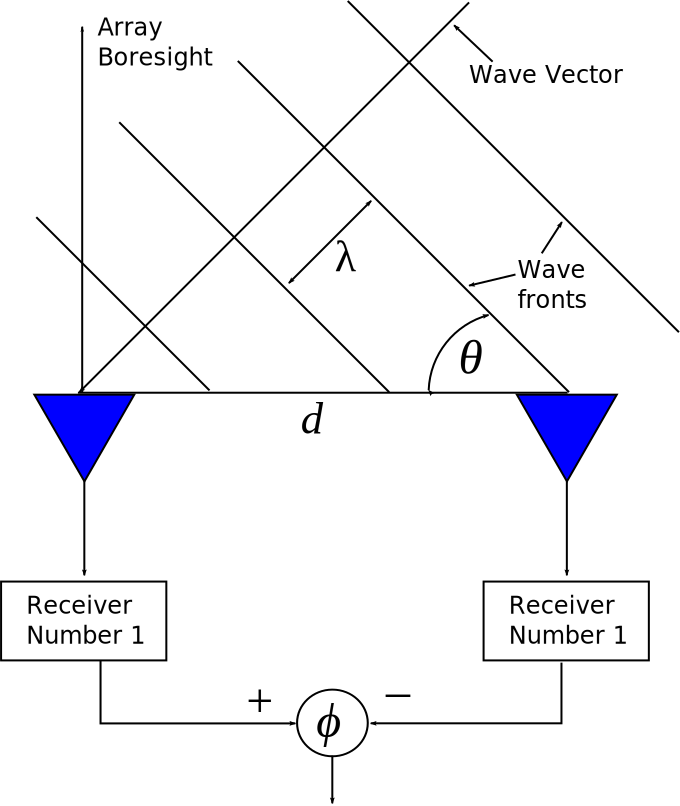
\includegraphics[width=0.4\textwidth]{lit_review/two_element_phase_df_model.pdf}
   \caption{Two-element phase interferometry. Note that as the element spacing (d) is more than half a wavelength there is ambiguity.}
   \label{fig:lit-two-element-phase}
\end{figure}

There are generally three subclasses of phase interferometry systems\cite{jenkins1991smallaperture}:
\begin{description}
  \item [Continuous phase measurement:] A single receiver takes in all of the antenna signals and compares the instantaneous phase of the signals, typically using analogue multipliers. It's fast and relatively simple for two antennas, but becomes complex as the number of elements increases and hence typically has a limited field of view, is susceptible to interference and is not very accurate.
  \item [Phase scanning correlation:] Here, a phase shifter and correlator are used. The phase shifter is varied until the correlator produces a peak output. Again, this is simple for two antennas but becomes complex when multiple phase shifters need to be varied. It is also slow as the phase shift needs to be swept to find the peak correlator output.
  \item [Fourier transform method:] The received signals are digitised and converted to frequency domain, where phase difference measurements are easily taken. As this is a digital technique, spectral processing can be done providing 20 dB to 30 dB of additional sensitivity over the other techniques. Also, working with digital signals in the frequency domain means that phase errors in the signal path can easily be compensated for and adjacent frequency signals can be ignored.
\end{description}
Should the antenna array contain more that two elements, the system either needs to switch between pairs of antennas if it wants to maintain a simple two-input receiver, or it needs a more advanced receiver to sample all antennas simultaneously. The Fourier transform method is the easiest to extend to having more antenna inputs, as the computation is done in the digital domain. Having all antennas processed by the receiver simultaneously allows for a faster system as no switching is required and also provides better performance as it can average multiple inputs at once. However, more inputs requires more computation and algorithmic complexity.

\section{Subspace and Statistical Techniques}
This class of techniques attempts to perform eigen analysis, decomposing the spectral or covariance matrix into eigen subspaces for noise and subspaces for signal. In some sense this equates to a beamforming algorithm which attempts to find an angle resulting in the strongest signal. 
Statistical methods generally involve taking snapshots of the signals received at each sensor, \(\vec{r}(t)\) and then calculating the covariance matrix of the received data\cite{poisel2012electronic}.

The advantage of working with multiple subspaces for each signal is that it allows direction finding to take place when there are multiple overlapping signals arriving at the array. Assume there are \(D\) narrow band signal all with unknown AoA parameter arriving at an \(M\) element array in the presence of uncorrelated noise, the problem space can be reduced from \(M\)-dimensional to \(D\)-dimensional\cite{van2004detection}.

It can be shown that the covariance matrix is diagonal for incoherent sources, non-diagonal and non-singular\footnote{A singular matrix is one which is not invertible, meaning the determinant is 0} for partially coherent sources and non-diagonal and singular if at least one of the sources are coherent\cite{poisel2012electronic}. 

Examples of these techniques include\cite{van2004detection}:
\begin{itemize}
  \item Spectral MuSiC (Multiple Signal Classification) which gets multiple signal snapshots to produce an estimated spectral matrix, \(\hat{\mathbf{S}}_{\mathbf{x}}\) and requires knowing the antenna array manifold vector. It can be applied to arbitrary arrays and performs best when the received signals are uncorrelated. The technique does not work when receiving multiple coherent signals.
  \item Root MuSiC, which is a special form of MuSiC allowing simplified polynomial equations provided linear arrays are used, and requires a lower antenna SNR than Spectral MuSiC.
  \item Least Squares and Total Least Squares ESPRIT (Estimation of Signal Parameter via Rotational Invariance Techniques) which constructs identical subarrays from uniform linear arrays, exploiting shift invariance properties of the array. It can be shown that the signal subspace eigenvectors are linear combinations of the array manifold vector. The RMS error for these techniques can be very close to the Cramer-Rao bound for estimation error\cite{van2004detection}.
\end{itemize}
These subspace techniques typically requires knowledge of the number of unique signals, \(D\), being received as they depend on being able to construct \(D\) subspaces. Seeing as coherent signals degrade performance, they suffer from multipath interference.

\section{Radiometer}
A radiometer is a device which is able to provide a very high accuracy approximation of noise power by averaging a large number of noise samples over a long time period. Due to the high accuracy measurements it can make, it is able to detect small changes in received power. 
It does this by achieving a high sensitivity. Sensitivity is the measure of how weak a signal and instrument is able to detect.

We will define power in terms of a matched load heated to a certain temperature observed over a certain bandwidth.
\begin{equation}
  P = kTB
\end{equation}
where \(k \approxeq \SI{1.38e-23}{\joule\per\kelvin}\), the Boltzmann constant. 

System temperature is a combination of noise powers from atmospheric emissions, the warm earth, the cosmic microwave background, receiver noise figure, losses in the RF chain and others. These noise sources mask the RFI signal which we are trying to locate. While typically an RFI signal below the noise floor would not be an issue, in the case of a radio astronomy reserver that signal will in all likelihood still be a problem because the noise floor of the MeerKAT array is so much lower than the RFI DF instrument. In essence, a signal which will be very loud to the telescope may be difficult for the DF system to even detect. Effort will hence need to go into ensuring that this instrument being designed will be able to see signals below its own noise floor. 

As the noise at an antenna is a combination of a multitude of noise sources, the central limit theorem states that output of the antenna will be approximately a normal (Gaussian) distribution. 

The noise temperature is defined as the noise power per unit bandwidth over the Boltzmann constant:
\begin{equation}
  T_N = \frac{P_v}{k}
\end{equation}

Assuming the power of a noise source remains constant, a single sample of the noise source has an RMS error of approximately \(\sqrt{2}T_{sys}\). However, by integrating the noise power from a certain bandwidth \(\Delta B\) over some integration time \(\tau\) the error can be significantly reduced to
\begin{equation}
  \sigma_{T} = \frac{\sqrt{2}T_{sys}}{\sqrt{2B\tau}} = \frac{T_{sys}}{\sqrt{B \tau}}
\end{equation}
Where \(\sigma_{T}\) is the RMS error in the measurement of the noise temperature, \(T\), and \(T_{sys}\) is the actual system noise temperature. Note that \(2B\tau\) is the number of samples acquired

This process used in a radiometer of acertaining a high accuracy approximation of a received signal by integrating the signal over some observation period can also be used in the context of a direction finding system. For this application, a long observation period may be used to extract a weak signal which is burried in noise so that the weak signal may be processed.

\begin{equation}
  \frac{S}{N} = \frac{S}{N}\sqrt{B\tau}
\end{equation}

Tsys = Tsky + Trx where Tsky is thestuff above and Trx is Johnson noise from electronic components. Tsky can't do anything about. Trx lowered by cooling components. 
The Trx is as a result of the Johnson-Nyquist noise. 

Extension to interferometry:

\(SEFD / (N(N-1))/2 \tau 2B)\)

Sources: \url{https://casper.berkeley.edu/astrobaki/index.php/Radiometer_Equation}
\url{https://casper.berkeley.edu/astrobaki/index.php/Radiometer_Equation_Applied_to_Telescopes}
\url{https://www.cv.nrao.edu/course/astr534/Radiometers.html}

